\chapter{Реалізація алгоритмів}             
            
    \section {Тестові дані}
            Для перевірки алгоритмів використовувались синтетичні набори даних. Була написана програма, що створює набір даних заданої форми. Утиліта зчитує із вказаного файла послідовно інформацію про центр групи об'єктів і дозволені відхилення від центру по кожній координаті та генерує вказану кількість об'єктів, розташованих випадковим чином у вказаних межах навколо центра. Задавши достатню кількість центральних точок і вибравши відповідні відхилення, можна отримати набір даних довільної форми. Зокрема, задавши центр групи приблизно посередині між усіма іншими точками, і досить великі відхилення по усіх координатах, можна досягнути ефекту шуму в даних ("зоряне небо"). Як і основна програма, утиліта написана на С++.
            
               
        \section {Програмне забезпечення}
            Для перевірки ефективності вищеописаних алгоритмів була створена їх програмна реалізація. У виборі мови програмування я керувався міркуваннями швидкодії та можливості контролю ресурсів комп'ютера. Вибір зупинився на С++. Реалізація являє собою консольну програму без графічного інтерфейсу, що зчитує дані з файла та зберігає у файлі результати кластеризації.
            
            %\begin{figure}
            %    \centering
            %    \includegraphics[scale=0.5]{chapters/03-software/Magister.png}
            %    \caption{Компонентна діаграма розробленого програмного забезпечення.}\label{fig:modules}
            %\end{figure}
            
            Створено об'єктно-орієнтовану модель для зберігання об'єктів вибірки. Для зберігання власне даних використовуються стандартні колекції STL. Де-юре STL не належить до стандарту мови С++, але де-факто усі сучасні поширені компілятори мають підтримку цеї бібліотеки. Перша версія програми включала об'єкт ,,DataContainer'', який містив асоціативний контейнер std::map, що дозволяв звертатись до обєктів вибірки по ідентифікатору. Кожен елемент вибірки був екземпляром класу Object, що містив std::vector вказівників на об'єкти класу Attribute. Кожен екземпляр Attribute містив числове значення відповідного атрибута та інформацію при присутність даного атрибута у відповідного об'єкта вибірки.
            
            Реалізовано також абстрактний клас AbstractMetric, який відповідав метриці простору. Архітектура програми дозволяє реалізувати довільну метрику простору. Таким чином при реалізації власне алгоритму кластеризації стало можливим абстрагуватись від типу метрики за допомогою механізму поліморфізму, доступного у С++. На даний момент із метрик реалізовано найпопулярнішу евклідову метрику.
            
            Написання програми відбувалось у текстовому редакторі vim. Для компіляції програми обрано компілятор gcc. Відлагодження програми відбувалось за допомогою набору інструментів gdb. Відслідковування витрат пам'яті та профілювання програми здійснювалось за допомогою valgrind. При розробці використовувалась система контролю версій git.
            
            Запуски програми та заміри часу проводились на комп’ютері із двоядерним процесором Intel Pentium D з тактовою частотою 2.8 ГГц. На комп’ютері встановлено 3 Гб оперативної пам’яті типу DDRII, що працює на частоті 667 МГц.
            
            Компіляція виконувалась із вказанням рівня автоматичної оптимізації -O3, в конфігурації Release.
            
            \subsection{K-means}
            
                K-means --- ітераційний алгоритм, тому час його роботи залежить не лише від об’єму вхідних даних, а і від їх структури. Тому оцінити загальний час роботи алгоритму складно. Натомість будемо оцінювати швидкодію конкретної реалізації за часом виконання одної ітерації. 
                
                На кожній ітерації k-means здійснюється обчислення центроїди кожного кластера, та обчислення відстані від кожного об’єкта до кожної центроїди. Оскільки на кожній ітерації кожен об’єкт повинен увійти в кластер, сумарна складність обчислення центроїд не змінюється між ітераціями. Кількість центроїд, очевидно, рівна кількості кластерів, тому час пошуку найближчої центроїди також залишається незмінним. Таким чином, час виконання ітерації на протязі усієї роботи алгоритму не змінюється. Це підтверджується графіком на рис.~\ref{fig:kmeans_linear}.
                
                
                
                \begin{figure}
                    \centering
                    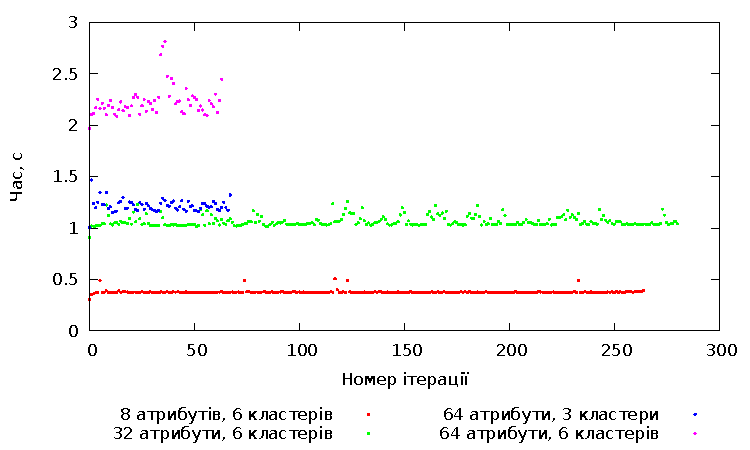
\includegraphics[scale=1.3]{kmeans_iteration_linear.pdf}
                    \caption{Графік залежності часу виконання ітерації k-means від її номера}\label{fig:kmeans_linear}
                \end{figure}
            
                     
